\Chapter{RESEARCH GENERAL WORKFLOW}\label{sec:Theme1}



My master research consisted of two different parallel projects. The first project consisted in a collaboration with the Linux Foundation and the second consisted of a case study of expertise evolution in the Linux Kernel.



\section{Srcmap}

In the interest of offering more visibility to the authors of the Linux Kernel, we built a data visualization tool capable of displaying a wide array of information about directories or file found in the linux git repository. We wanted to display the following data points about each file and directory of the source code:

\begin{itemize}
	\item Number of lines of code (LOC)
	\item Median age of the LOC within a file/directory
	\item Number of lines of code modified since 2016
	\item A list of the 20 developers with the most lines of code
	\item A bar plot displaying the distribution of line of code age
\end{itemize}

We needed an interface that would allow the user to navigate the different files and direcotries of Linux while displaying our list of datapoints, which is why we chose to base the tool on a treemap. Treemaps, which were introduced by Shneiderman~\citep{Bederson-2002} as a solution to display large hierarchical dataset on a 2 dimentional plane, were a great fit for our tool's requierments. 

\subsection{Srcmap 1.0}

In the first version of Srcmap\footnote{\url{http://mcis.polymtl.ca/~courouble/linux.html}}, we used the Google Chart treemap implementation\footnote{\url{https://developers.google.com/chart/interactive/docs/gallery/treemap}}. This easy to use library allowed us to create a quick proof of concept. 

\begin{figure}[htb]
\centering
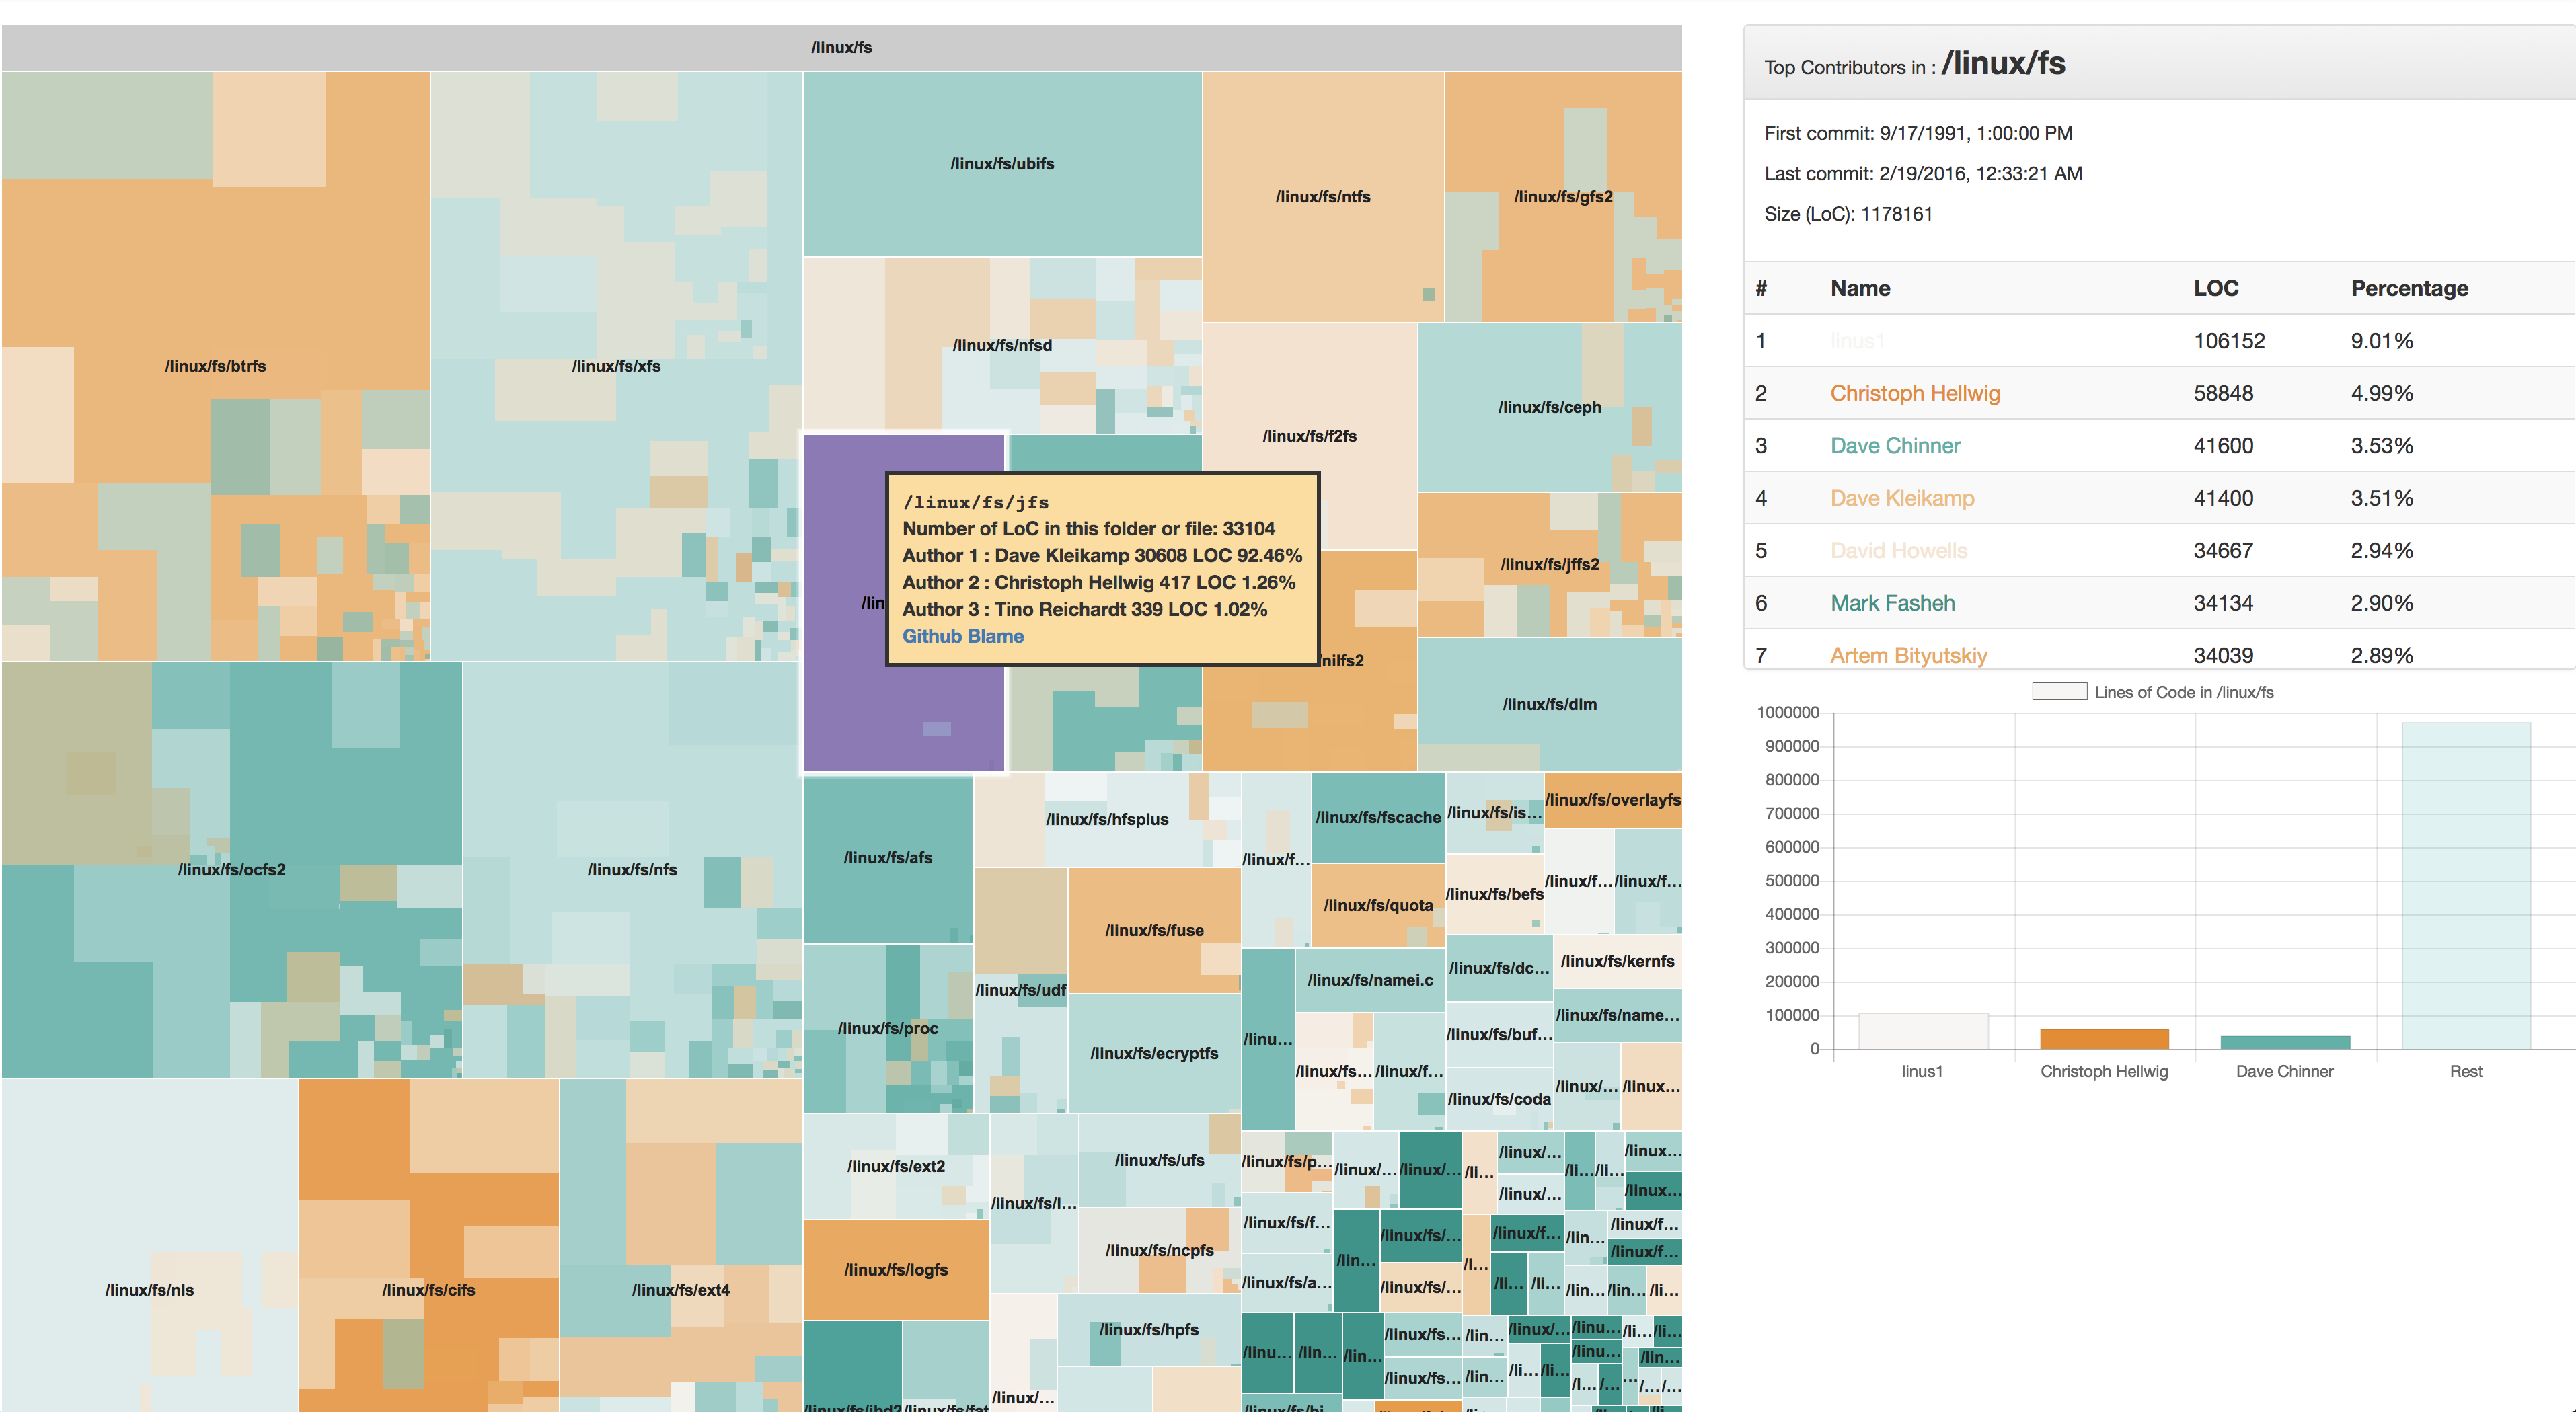
\includegraphics[width=5in]{srcmap1}
\caption{First version of srcmap}
\label{fig:srcmap1}
\end{figure}

\autoref{fig:srcmap1} shows the first version of Srcmap. The diferent boxes represent subdirectories of the Linux Kernel. The different colors present within each box give a preview of the content of the box. In this version of the tool, the color represents the developer having contributed the most lines of code in the contained files. Furthermore, the size of the boxes is proportional to the number of lines of code existing within the file or directory represented by the box. The panel on the right of the screen and the tooltip contain most of the data: exact number of lines of code, age of the first and last lines of code to be added, and the top 20 authors and their percentage of lines of code contributed.

Even though the library offered by Google allowed us to quickly provide a strong proof of concept, we discovered some limitations when we tried adding new features to the tool. The tool had issues handling the size of the dataset. The actual data would take up to 30 seconds to load, and navigating between each node became very slow. This is why we decided to create a new version of the tool with a different treemap library.


\subsection{Srcmap 2.0}


After some research, we discovered a new treemap implementation\footnote{\url{https://carrotsearch.com/foamtree/}} capable of handling large dataset and deeply nested stuctures, which we used for the second version of the tool\footnote{\url{http://mcis.polymtl.ca/~courouble/dev/}}. This new version introduced three important features: 
\begin{itemize}
	\item Coloring the files and directories according to three metrics:
	\begin{itemize}
		\item LOC
		\item Median age
		\item Number of commits since 2016, or "Hot files"
	\end{itemize}
	\item File search
	\item A plot displaying the age distribution of LOC present in the file/directory.
\end{itemize}


\begin{figure}[htb]
\centering
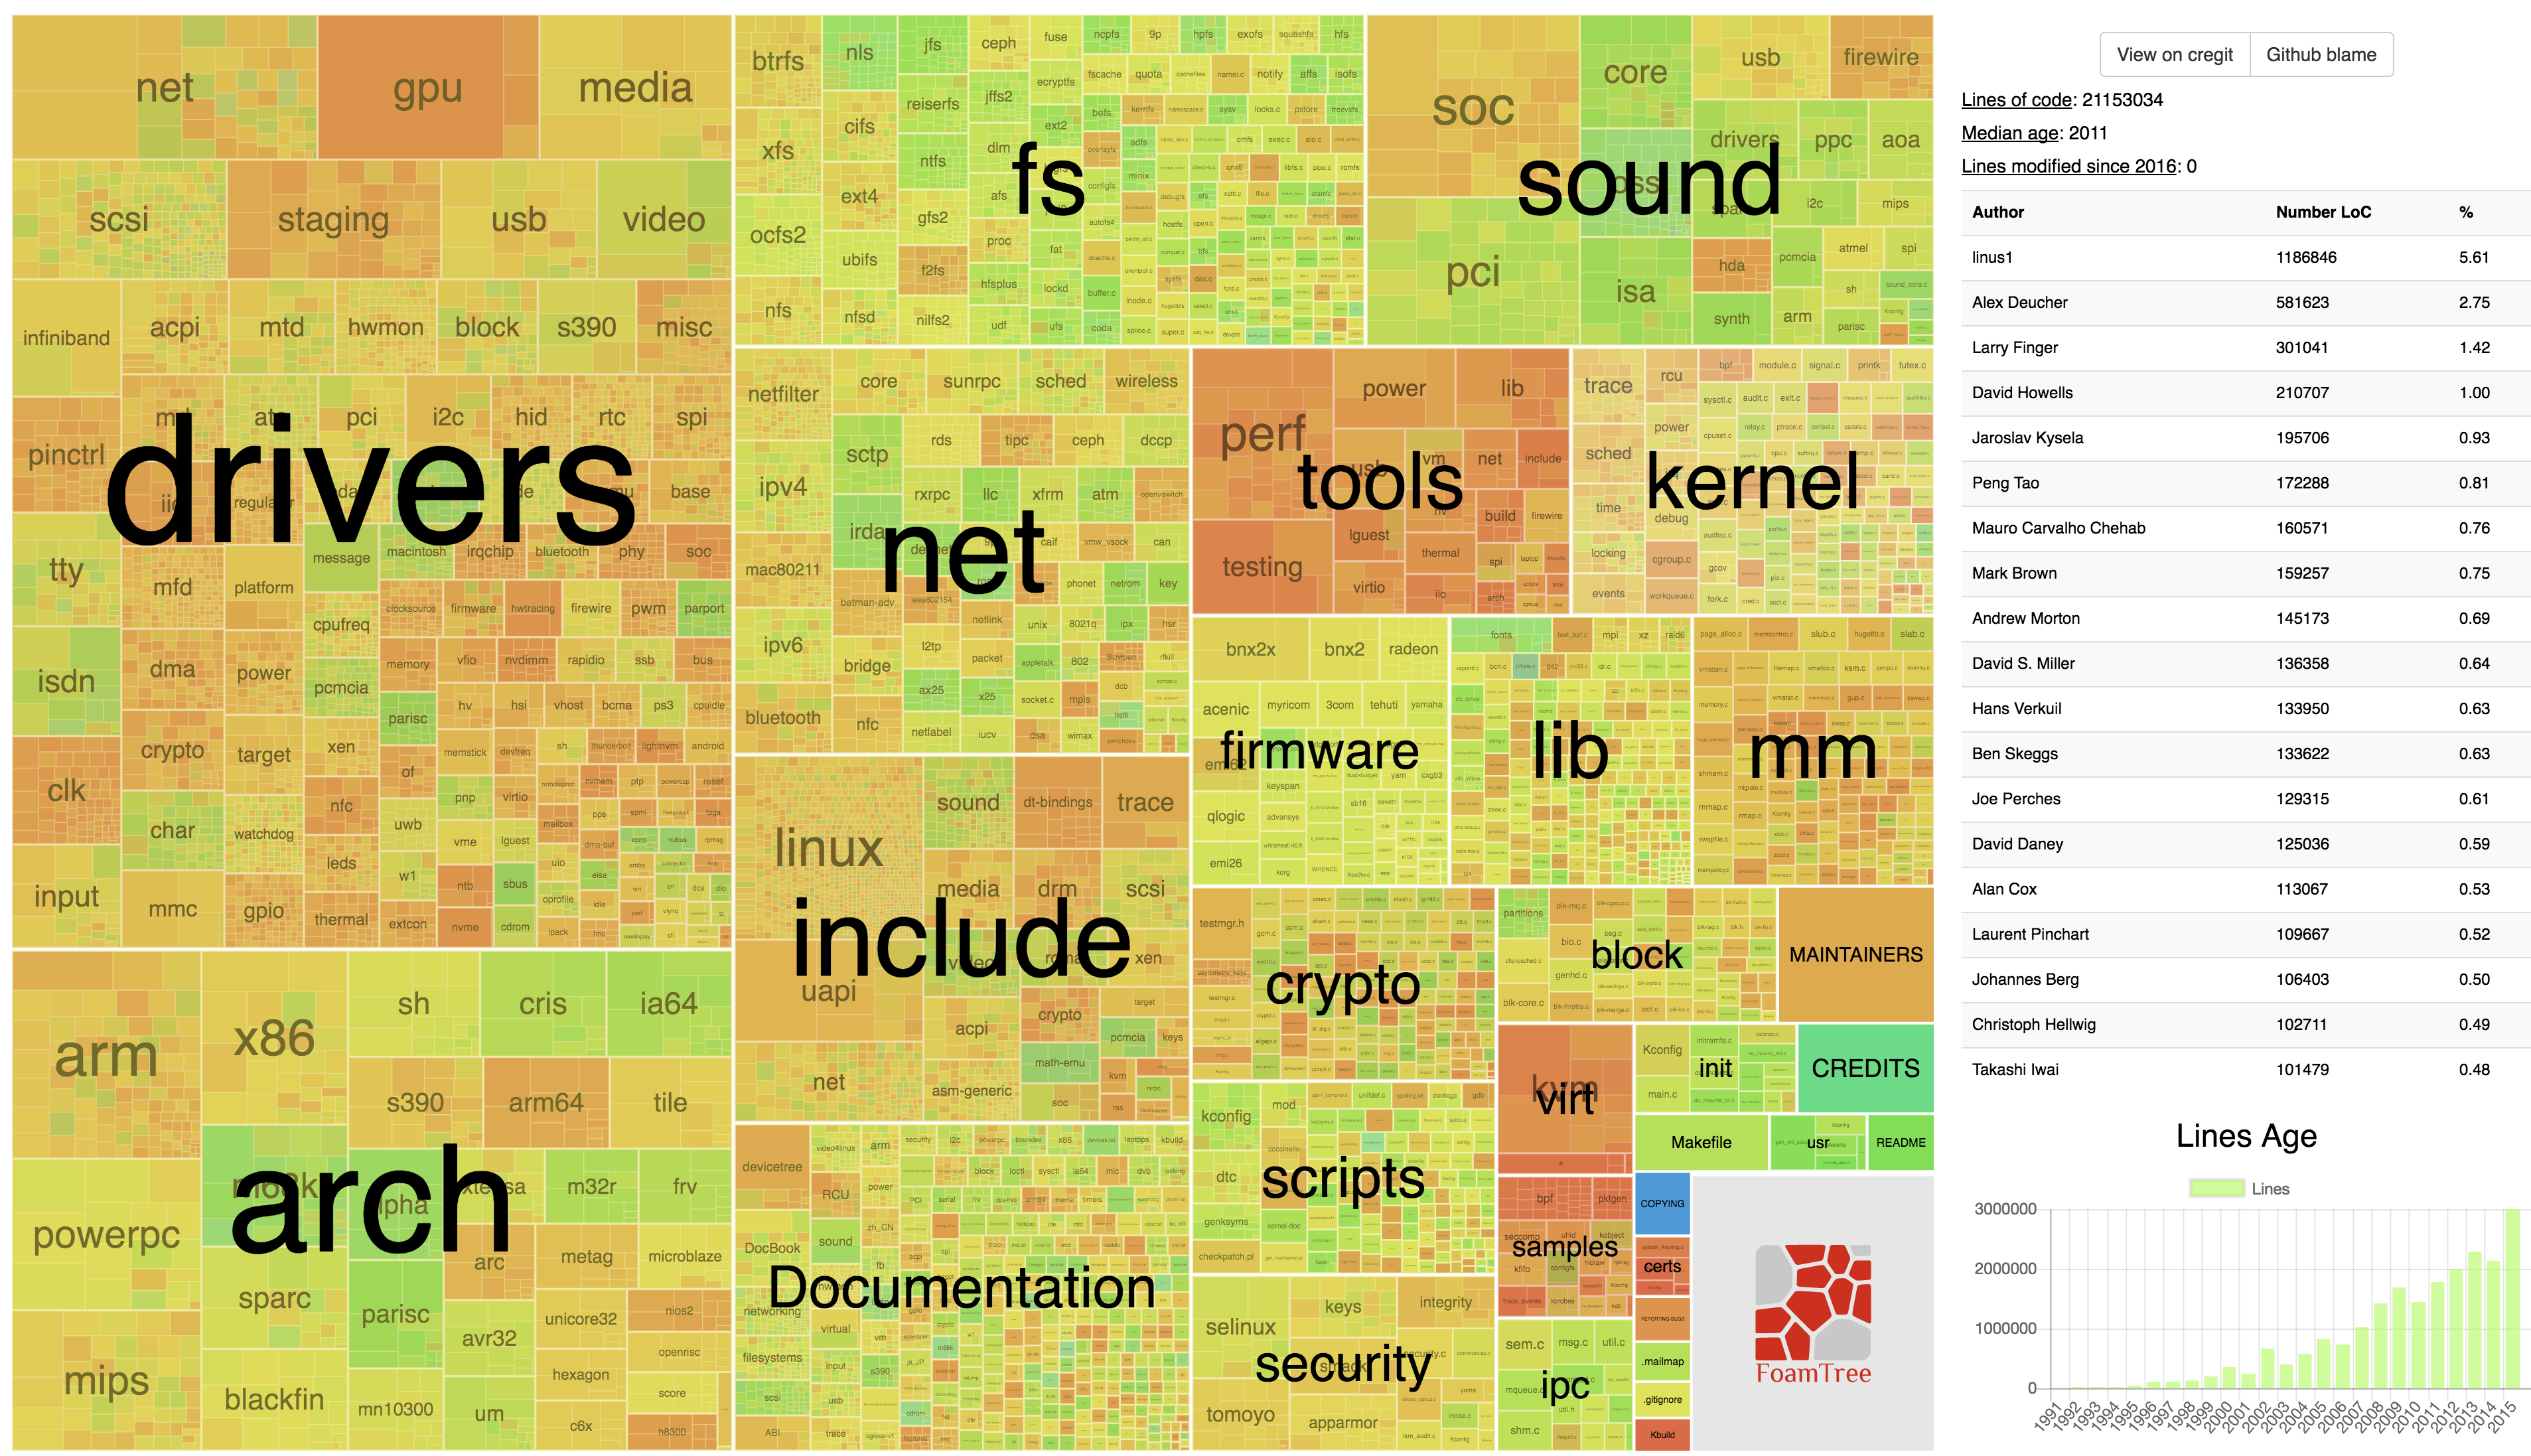
\includegraphics[width=5in]{srcmap2}
\caption{Second version of srcmap}
\label{fig:srcmap2}
\end{figure}

\section{Email2git}


\section{Integrating Email2git with Cregit}



% \begin{itemize}
% \item open source tools	
%   \begin{itemize}
% 	\item srcmap
% 	\item email2git
% 	\item integrating email2git with cregit
% 	\item traveling to conferences, talking to linux devs/maintainers, introducing the tools and getting feedback
% 	\item How email2git can help us with our research 
%   \end{itemize}	
% \item Reseach paper 
% \end{itemize}